\subsubsubsubsection{Speed Limit}
\begin{figure}[h]
\centering
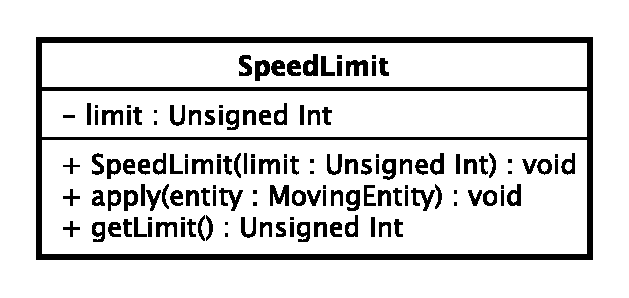
\includegraphics[scale=0.6,keepaspectratio]{images/solution/speed_limit.eps}
\caption{\pPassive::SpeedLimit}
\label{fig:sd-app-speed_limit}
\end{figure}
\FloatBarrier
\begin{itemize}
  \item \textbf{\descr} \\
It implements the speed limit road sign resetting the max speed valued of each moving entity.
  \item \textbf{\attrs}
  \begin{itemize}
    \item \texttt{limit: Unsigned Int} \\
The speed limit.
  \end{itemize}
  \item \textbf{\ops}
  \begin{itemize} 
  \item[+] \texttt{SpeedLimit(limit: Unsigned Int)} \\
Creates a speed limit road sign with a specific limit.    
  \item[+] \texttt{apply(entity: MovingEntity)} \\
Notifies the entity only if the entity max speed is greater than the limit.
The entity will update its maxSpeed according to the limit value.
  \item[+] \texttt{getLimit(): Unsigned Int} \\
Returns the limit value.
  \end{itemize}
\end{itemize}
